\documentclass[border=10pt]{standalone}
\usepackage{tikz}
\usetikzlibrary{arrows.meta, shapes, calc, fit, positioning, backgrounds}

\definecolor{tealfill}{RGB}{225,245,238}
\definecolor{tealstroke}{RGB}{15,110,86}
\definecolor{bluefill}{RGB}{230,241,251}
\definecolor{bluestroke}{RGB}{24,95,165}
\definecolor{purplefill}{RGB}{238,237,254}
\definecolor{purplestroke}{RGB}{83,74,183}
\definecolor{amberfill}{RGB}{250,238,218}
\definecolor{amberstroke}{RGB}{186,117,23}
\definecolor{textdark}{RGB}{40,40,38}
\definecolor{textsub}{RGB}{90,88,84}
\definecolor{attline}{RGB}{127,119,221}

\tikzset{
  block/.style={
    rectangle, rounded corners=8pt,
    minimum width=#1, minimum height=1.1cm,
    text width=#1-0.5cm,
    align=center,
    draw, thick,
    font=\sffamily
  },
  block/.default=8cm,
  label/.style={font=\sffamily\small\bfseries, text=textdark, draw=none, fill=none},
  sublabel/.style={font=\sffamily\footnotesize, text=textsub, draw=none, fill=none},
  sectionlabel/.style={font=\sffamily\tiny\scshape, text=textsub, draw=none, fill=none, opacity=0.7},
  arrow/.style={-{Stealth[length=6pt,width=5pt]}, thick, color=textsub},
  attarrow/.style={-{Stealth[length=5pt,width=4pt]}, color=attline},
}

\begin{document}
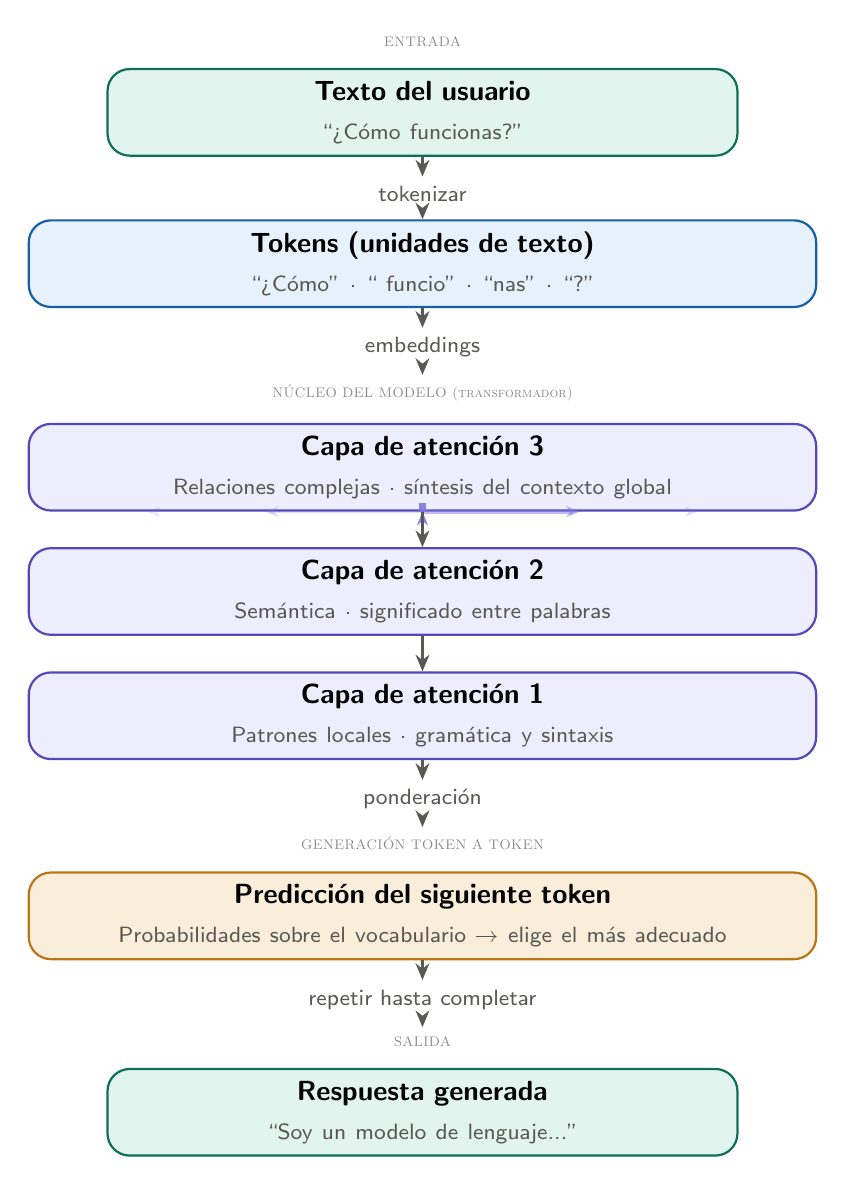
\begin{tikzpicture}[node distance=0.6cm]

%% ─── ENTRADA ───────────────────────────────────────────────
\node[sectionlabel] (sec1) {ENTRADA};

\node[block, below=0.15cm of sec1,
      fill=tealfill, draw=tealstroke]
  (entrada) {%
    \textbf{Texto del usuario}\\[2pt]
    \textcolor{textsub}{\footnotesize ``¿Cómo funcionas?''}
  };

%% Arrow + label
\node[sublabel, below=0.25cm of entrada] (lbl1) {tokenizar};
\draw[arrow] (entrada.south) -- (lbl1.north);

%% ─── TOKENS ─────────────────────────────────────────────────
\node[sectionlabel, below=0.1cm of lbl1] (sec2) {};

\node[block=10cm, below=0.1cm of lbl1,
      fill=bluefill, draw=bluestroke]
  (tokens) {%
    \textbf{Tokens (unidades de texto)}\\[2pt]
    \textcolor{textsub}{\footnotesize ``¿Cómo'' · `` funcio'' · ``nas'' · ``?''}
  };

%% Arrow + label
\node[sublabel, below=0.25cm of tokens] (lbl2) {embeddings};
\draw[arrow] (tokens.south) -- (lbl2.north);

%% ─── NÚCLEO ──────────────────────────────────────────────────
\node[sectionlabel, below=0.1cm of lbl2]
  (sec3) {NÚCLEO DEL MODELO (transformador)};

\node[block=10cm, below=0.15cm of sec3,
      fill=purplefill, draw=purplestroke]
  (capa3) {%
    \textbf{Capa de atención 3}\\[2pt]
    \textcolor{textsub}{\footnotesize Relaciones complejas · síntesis del contexto global}
  };

\node[block=10cm, below=0.45cm of capa3,
      fill=purplefill, draw=purplestroke]
  (capa2) {%
    \textbf{Capa de atención 2}\\[2pt]
    \textcolor{textsub}{\footnotesize Semántica · significado entre palabras}
  };

\node[block=10cm, below=0.45cm of capa2,
      fill=purplefill, draw=purplestroke]
  (capa1) {%
    \textbf{Capa de atención 1}\\[2pt]
    \textcolor{textsub}{\footnotesize Patrones locales · gramática y sintaxis}
  };

%% Attention weight lines inside capa3
\foreach \op/\xoff in {0.12/-3.5, 0.25/-2.0, 0.9/0, 0.5/2.0, 0.15/3.5}{
  \draw[attarrow, opacity=\op, line width=\op*3pt]
    ($(capa3.south)+(0,0)$) -- ($(capa3.south)+(\xoff cm,0)$);
}

%% Arrow + label
\node[sublabel, below=0.25cm of capa1] (lbl3) {ponderación};
\draw[arrow] (capa1.south) -- (lbl3.north);

%% ─── GENERACIÓN ──────────────────────────────────────────────
\node[sectionlabel, below=0.1cm of lbl3]
  (sec4) {GENERACIÓN TOKEN A TOKEN};

\node[block=10cm, below=0.15cm of sec4,
      fill=amberfill, draw=amberstroke]
  (gen) {%
    \textbf{Predicción del siguiente token}\\[2pt]
    \textcolor{textsub}{\footnotesize Probabilidades sobre el vocabulario → elige el más adecuado}
  };

%% Arrow + label
\node[sublabel, below=0.25cm of gen] (lbl4) {repetir hasta completar};
\draw[arrow] (gen.south) -- (lbl4.north);

%% ─── SALIDA ──────────────────────────────────────────────────
\node[sectionlabel, below=0.1cm of lbl4] (sec5) {SALIDA};

\node[block, below=0.15cm of sec5,
      fill=tealfill, draw=tealstroke]
  (salida) {%
    \textbf{Respuesta generada}\\[2pt]
    \textcolor{textsub}{\footnotesize ``Soy un modelo de lenguaje...''}
  };

%% ─── VERTICAL ARROWS ─────────────────────────────────────────
\draw[arrow] (lbl1.south) -- (tokens.north);
\draw[arrow] (lbl2.south) -- (sec3.north);
\draw[arrow] (capa3.south) -- (capa2.north);
\draw[arrow] (capa2.south) -- (capa1.north);
\draw[arrow] (lbl3.south) -- (sec4.north);
\draw[arrow] (lbl4.south) -- (sec5.north);

\end{tikzpicture}
\end{document}
